\subsection{Project Overview}
Student provides a high-level overview of the project in layman’s terms. Background information such as the problem domain, the project origin, and related data sets or input data is given.

The improvement on the camera and the widespread of larger capacity hardwares lead us to store more digital pictures. However computers can't understand the meaning of the pictures, so it is essential for us humans to classify or search images. Image recognition(Figure.\ref{fig:one}) will help us to classify or search pictures without our intervention. These days, because of the development of the computational capacity, we can process large number of pictures with high level accuracy(nearly the human's recognition). In this project, I'll discuss the image recognition algorithm which will be useful in the classification of large number of images.


\begin{figure}[htbp]

\begin{center}
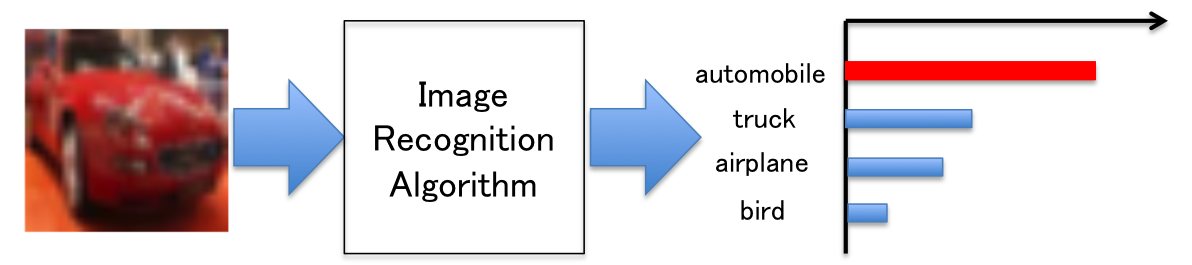
\includegraphics[width=10cm]{picture/Image_Recognition.png}
\end{center}
\caption{Image of the Algorithm}
\label{fig:one}

\end{figure}

